
\documentclass{article}

% Use preprint option for arXiv submission
\usepackage[preprint]{neurips_2026}

\usepackage[utf8]{inputenc} % allow utf-8 input
\usepackage[T1]{fontenc}    % use 8-bit T1 fonts
\usepackage{hyperref}       % hyperlinks
\usepackage{url}            % simple URL typesetting
\usepackage{booktabs}       % professional-quality tables
\usepackage{amsfonts}       % blackboard math symbols
\usepackage{amsmath}        % math environments
\usepackage{amssymb}        % additional math symbols
\usepackage{nicefrac}       % compact symbols for 1/2, etc.
\usepackage{microtype}      % microtypography
\usepackage{xcolor}         % colors
\usepackage{graphicx}       % include graphics

\title{Analyzing the Nonlocality of Sparse Autoencoder Features}

\author{%
  Xiao-Liang Qi \\
  Stanford Institute for Theoretical Physics\\
  Stanford University\\
  Stanford, CA 94305 \\
  \texttt{xlqi@stanford.edu} \\
}

\begin{document}

\maketitle

\begin{abstract}
    Sparse autoencoders (SAEs) have emerged as a powerful tool for extracting
    interpretable features from the internal representations of large language
    models (LLMs). Motivated by an analogy with holographic duality in
    theoretical physics, where strongly correlated boundary degrees of freedom
    map to weakly coupled bulk fields of varying nonlocality, we introduce a
    gradient-based entropy measure that quantifies how nonlocal each SAE
    feature is in the input token space. For a given feature at a given layer,
    we compute the Jacobian of the feature activation with respect to all input
    token embeddings, normalize the resulting influence distribution, and
    evaluate its Shannon entropy. Applying this measure to Pythia-70m-deduped
    with pretrained SAEs across six transformer layers, we find that:
    (i)~features exhibit a broad distribution of nonlocality;
    (ii)~deeper layers produce systematically more nonlocal features;
    (iii)~the entropy of individual features saturates with increasing context
    length, indicating a finite effective support; and
    (iv)~SAE features generally have lower entropy than the reconstructed token
    vectors, supporting the view that sparse features provide a low-entropy
    decomposition of the residual stream.
\end{abstract}

%=============================================================================
\section{Introduction}
\label{sec:introduction}
%=============================================================================

Large language models (LLMs) based on the transformer architecture achieve
remarkable performance across a wide range of natural language tasks, yet
their internal representations remain poorly understood. A central challenge
in mechanistic interpretability is to decompose the dense,
high-dimensional activations of a transformer into meaningful,
human-interpretable units~\citep{bricken2023monosemanticity,
    templeton2024scaling}.

Sparse autoencoders (SAEs) offer a promising approach to this
problem~\citep{yun2021transformer, cunningham2023sparse,
    bricken2023monosemanticity, templeton2024scaling}. An SAE consists of a
nonlinear encoder $f = E(y)$ that maps an internal activation vector
$y \in \mathbb{R}^d$ to a higher-dimensional feature vector
$f \in \mathbb{R}^M$ (with $M \gg d$), together with a linear decoder
that approximately reconstructs the original activation. The encoder
typically applies a ReLU nonlinearity,
\begin{equation}
    \label{eq:encoder}
    f_a = \operatorname{ReLU}\!\Bigl(\sum_{\mu} W^{\mathrm{enc}}_{a\mu}\, y_\mu + b^{\mathrm{enc}}_a
    \Bigr),
\end{equation}
where the sparsity of $f$ is enforced through an $L_1$ penalty during
training~\citep{ranzato2007sparse, ng2011sparse}. The decoder is a linear
map,
\begin{equation}
    \label{eq:decoder}
    \tilde{y}_\mu = \sum_a D_{\mu a}\, f_a\,,
\end{equation}
satisfying $\tilde{y} \simeq y$. Although $\dim(f) > \dim(y)$, the
sparsity constraint ensures that only a small number of features are active
for any given input, so the SAE still performs a form of compression.

In a causal transformer, the residual stream activation at position~$t$
and layer~$n$ is denoted $y_t^{(n)}$. The attention mechanism gives
$y_t^{(n+1)} = \operatorname{Attn}_n(y_{t' \le t}^{(n)})$,
so that deeper layers can integrate information from progressively more
input tokens. An SAE trained on a particular layer produces per-position
feature vectors $f_t^{(n)} = E_n(y_t^{(n)})$, and the resulting features
have been shown to correspond to interpretable concepts such as named
entities, syntactic patterns, and semantic
categories~\citep{bricken2023monosemanticity, templeton2024scaling}.

In this work, we introduce a gradient-based entropy measure that quantifies
the \emph{nonlocality} of each SAE feature in the input token space---that
is, how many input tokens significantly influence a given feature
activation. We perform a systematic numerical study across all layers and
context lengths of a small transformer model (Pythia-70m-deduped), and we
compare the nonlocality of individual features with that of the full token
vector. Our main findings are:
\begin{itemize}
    \item SAE features exhibit a broad distribution of nonlocality, with
          entropy ranging from less than one bit to over five bits.
    \item Deeper layers produce systematically more nonlocal features,
          consistent with encoding more abstract concepts.
    \item Feature entropy saturates with increasing context length,
          indicating a finite effective support for each feature.
    \item Individual features generally have lower entropy than the
          reconstructed token vector, supporting the interpretation that
          the residual stream is a superposition of features with different
          nonlocality scales.
\end{itemize}

%=============================================================================
\section{Analogy with holographic duality}
\label{sec:holography}
%=============================================================================

Our approach is motivated by a structural analogy between SAE features and
bulk fields in the Anti-de~Sitter/Conformal Field Theory (AdS/CFT)
correspondence~\citep{maldacena1999large, qi2018spacetime}. In holographic
duality, a strongly correlated conformal field theory on the boundary of an
anti-de~Sitter spacetime is dual to a gravitational theory in the bulk.
The bulk theory is weakly coupled in the semiclassical limit, and its
local fields can be reconstructed as nonlocal functionals of boundary
operators via the HKLL prescription~\citep{hamilton2006holographic}.
Crucially, different bulk fields live at different radial depths: fields
deeper in the bulk correspond to more nonlocal combinations of boundary
operators. The Ryu--Takayanagi formula~\citep{ryu2006holographic} further
connects bulk geometry to boundary entanglement entropy, establishing a
deep link between information-theoretic quantities and emergent spatial
structure.

SAE features share three key structural properties with holographic bulk
fields:
\begin{enumerate}
    \item \textbf{Nonlocality.} Each SAE feature at an internal layer
          depends on multiple input tokens through the attention mechanism,
          just as a bulk field depends nonlocally on boundary operators.
    \item \textbf{Approximate independence.} Well-trained SAE features are
          approximately uncorrelated for the natural distribution of inputs,
          analogous to the emergent locality of weakly coupled bulk fields.
    \item \textbf{Sparsity.} Only a small number of features are active for
          any given input, paralleling the semiclassical regime where the
          number of bulk excitations is small.
\end{enumerate}

This analogy suggests that different SAE features---corresponding to
concepts at different levels of abstraction (e.g., individual words versus
semantic categories such as ``fruit'' or ``animal'')---should exhibit
different degrees of nonlocality in the input token space. If this is the
case, one can assign to each feature a ``depth'' in an emergent radial
dimension, with more abstract and nonlocal features sitting deeper. The
primary goal of this paper is to test this picture quantitatively by
measuring the nonlocality of SAE features across transformer layers.

%=============================================================================
\section{Methodology}
\label{sec:methodology}
%=============================================================================

Motivated by the holographic analogy of Section~\ref{sec:holography}, we
seek a quantitative measure of how nonlocally each SAE feature depends on
the input tokens. In holographic duality, the nonlocality of a bulk field
is characterized by how it is reconstructed from boundary operators; here,
we characterize the nonlocality of a feature by how its activation depends
on the input token embeddings, as measured through the gradient.

\subsection{Gradient-based influence measure}
\label{sec:influence}

Consider a feature $f_a$ at token position~$t$ and layer~$n$ in a causal
transformer. Due to the causal attention mask, $f_a(t,n)$ can depend on
all input token embeddings $x_{\mu,t'}$ with $t' \le t$, where
$\mu = 1, \ldots, d_{\mathrm{model}}$ indexes the components of the
embedding vector. We define the \emph{influence matrix} as the Jacobian
of the feature activation with respect to the input embeddings:
\begin{equation}
    \label{eq:influence_matrix}
    I_{a,\mu}(t,n \mid t')
    = \frac{\partial f_a(t,n)}{\partial x_{\mu,t'}}\,,
    \qquad t' \le t.
\end{equation}
The squared Frobenius norm over the embedding index defines the
\emph{influence strength} of token~$t'$ on feature~$a$:
\begin{equation}
    \label{eq:influence_strength}
    J_a(t,n \mid t')
    = \sum_{\mu=1}^{d_{\mathrm{model}}}
        [I_{a,\mu}(t,n \mid t')]^2.
\end{equation}
By construction, $J_a(t,n \mid t') \ge 0$ for all~$t'$. We choose the
squared $L_2$ norm so that the total influence is additive:
\begin{equation}
    \label{eq:total_influence}
    J_{a,\mathrm{tot}}(t,n)
    = \sum_{t' \le t} J_a(t,n \mid t').
\end{equation}

\subsection{Entropy of influence distribution}
\label{sec:entropy}

We normalize the influence strength to obtain a probability distribution
over input token positions:
\begin{equation}
    \label{eq:prob}
    p(t') = \frac{J_a(t,n \mid t')}{J_{a,\mathrm{tot}}(t,n)}\,.
\end{equation}
The \emph{influence entropy} is then the Shannon entropy of this
distribution, measured in bits:
\begin{equation}
    \label{eq:entropy}
    S_a(t,n) = -\sum_{t'} p(t') \log_2 p(t').
\end{equation}
The quantity $2^{S_a}$ gives the effective number of input tokens that
significantly influence feature~$a$. A feature that depends on only a
single token has $S_a = 0$, while a feature that depends uniformly on all
$L$~tokens has $S_a = \log_2 L$.

In practice, we evaluate the entropy at the last token position $t = L$ of
each input batch, since this position has access to all preceding tokens
through the causal attention mask. For each feature, we average $S_a$ over
all batches in which the feature is active (i.e.,
$f_a > \text{threshold}$). Alternative measures such as the inverse
participation ratio $(\sum_{t'} p(t')^2)^{-1}$ are also possible but are
not explored in this work.

\subsection{Token vector entropy for comparison}
\label{sec:token_entropy}

To assess whether SAE features provide a ``low-entropy decomposition'' of
the residual stream, we compare the influence entropy of individual
features with that of the full reconstructed token vector. Recalling the
decoder in Eq.~\eqref{eq:decoder},
\begin{equation}
    \label{eq:decoder_decomp}
    \tilde{y}_\mu
    = \sum_a D_{\mu a}\, f_a
    = D_{\mu a_1} f_{a_1} + D_{\mu a_2} f_{a_2} + \cdots\,,
\end{equation}
the Jacobian of the reconstructed vector with respect to the input
embeddings is
\begin{equation}
    \label{eq:token_jacobian}
    \frac{\partial \tilde{y}_\nu(t,n)}{\partial x_{\mu,t'}}
    = \sum_a D_{\nu a}
    \frac{\partial f_a(t,n)}{\partial x_{\mu,t'}}\,.
\end{equation}
We define the token vector influence as
\begin{equation}
    \label{eq:token_influence}
    R(t,n \mid t')
    = \sum_{\nu,\mu}
    \left(\frac{\partial \tilde{y}_\nu(t,n)}{\partial x_{\mu,t'}}\right)^{\!2},
\end{equation}
where the sum runs over both output component~$\nu$ and input
component~$\mu$. Normalizing
$q(t') = R(t,n \mid t') \big/ \sum_{t'} R(t,n \mid t')$ and computing
the Shannon entropy yields the token vector entropy. Since $\tilde{y}$ is
a superposition of features with potentially different nonlocality scales,
we expect the token vector entropy to be higher than the entropy of typical
individual features.

%=============================================================================
\section{Experimental setup}
\label{sec:setup}
%=============================================================================

\paragraph{Model.}
We use Pythia-70m-deduped~\citep{biderman2023pythia}, a 6-layer causal
transformer with hidden dimension $d_{\mathrm{model}} = 512$, trained on
the deduplicated Pile dataset.

\paragraph{Sparse autoencoders.}
We use pretrained SAEs from the \texttt{dictionary\_learning}
library~\citep{marks2024dictionary}, with $M = 32{,}768$ latent features
per layer. Separate SAEs are trained for the residual stream output at each
of the six layers (\texttt{resid\_out\_layer0} through
\texttt{resid\_out\_layer5}).

\paragraph{Dataset.}
All analyses are performed on the WikiText-2 training
set (${\sim}$1M~tokens). Input batches are constructed by taking contiguous
sequences of tokens from the corpus.

\paragraph{Hyperparameters.}
The default batch size (context length) is $L = 64$ tokens. For the
context-length dependence study (Section~\ref{sec:length}), we vary $L$
from 8 to 128. A feature is considered active in a given batch if its
activation exceeds a threshold of $0.2$.

\paragraph{Leading features.}
We define \emph{leading features} as those whose activation frequency
(fraction of token positions where the feature is active) exceeds $0.1\%$
across the dataset. At each layer, the top 500 features by activation
frequency are selected for detailed analysis.

\paragraph{Gradient computation.}
For each batch, we perform a forward pass through the transformer and SAE
with gradient tracking enabled on the input embeddings. The influence
$\partial f_a(L,n) / \partial x_{\mu,t'}$ is computed for all active
leading features~$a$ and all positions $t' \le L$ using PyTorch
\texttt{autograd}. The token vector influence
(Eq.~\eqref{eq:token_influence}) is computed using
\texttt{torch.autograd.functional.jacobian} for the full Jacobian matrix.

%=============================================================================
\section{Results}
\label{sec:results}
%=============================================================================

\subsection{Feature sparsity statistics}
\label{sec:sparsity}

Before analyzing nonlocality, we verify that the SAE features exhibit the
expected sparsity structure. Figure~\ref{fig:unique_tokens} shows the
distribution of the number of unique tokens that activate each feature at
layer~0. The distribution is heavy-tailed: the vast majority of features
activate on very few tokens, while a small number of features activate
broadly across thousands of unique tokens.

\begin{figure}[t]
    \centering
    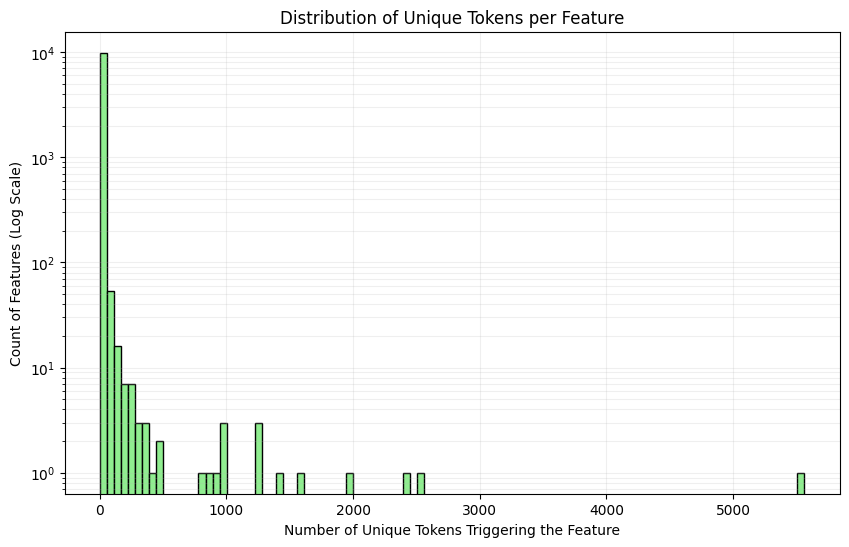
\includegraphics[width=0.72\linewidth]{figures/unique_tokens_histogram.png}
    \caption{Distribution of the number of unique tokens activating each
        feature (layer~0). The vertical axis is on a logarithmic scale. The
        distribution is heavy-tailed, with most features activating on very few
        tokens and a small number activating on thousands of unique tokens.}
    \label{fig:unique_tokens}
\end{figure}

To verify the approximate independence of features, we compute the
correlation matrix
$C_{ab} = \langle A^a A^b \rangle - \langle A^a \rangle \langle A^b
    \rangle$, where $A^a$ is the binary activation indicator for feature~$a$.
As shown in Fig.~\ref{fig:correlation}, the matrix is approximately
diagonal, confirming that the SAE features are approximately independent
under the natural text distribution.

\begin{figure}[t]
    \centering
    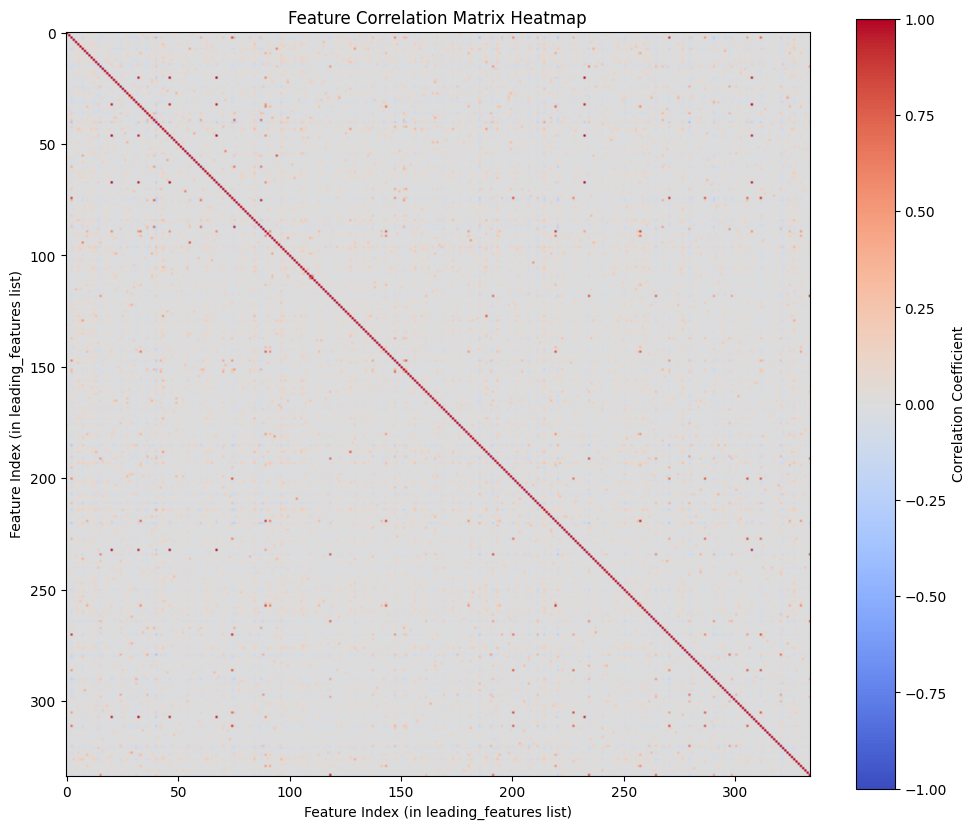
\includegraphics[width=0.62\linewidth]{figures/correlation_heatmap.png}
    \caption{Feature correlation matrix $C_{ab}$ for leading features at
        layer~3. The matrix is approximately diagonal, confirming approximate
        independence of SAE features under the natural text distribution. A
        small number of off-diagonal entries with elevated correlation are
        visible.}
    \label{fig:correlation}
\end{figure}

\subsection{Influence distribution and entropy}
\label{sec:influence_results}

For each active feature at the last token position, we compute the
influence strength $J_a(t,n \mid t')$ across all input positions.
Figure~\ref{fig:influence_heatmap} shows the influence distribution for
Feature~531 at layer~3, computed over 45~batches in which the feature was
active. The influence is structured and non-uniform: certain input
positions contribute significantly more than others, and the variance
across batches is substantial but the mean profile shows clear structure.

\begin{figure}[t]
    \centering
    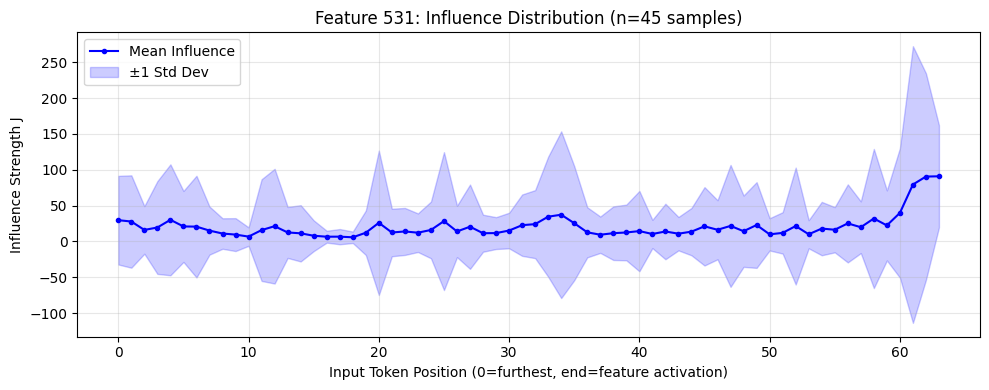
\includegraphics[width=0.88\linewidth]{figures/influence_heatmap_0.png}
    \caption{Influence distribution $J_a(t,n \mid t')$ for Feature~531
        across 45~batches at layer~3. The horizontal axis is the input token
        position ($0 =$ furthest from the feature activation,
        end $=$ feature position). The blue curve shows the mean influence with
        $\pm 1$~standard deviation (shaded). The feature shows structured,
        non-uniform dependence on input tokens, with elevated influence near
        the feature position.}
    \label{fig:influence_heatmap}
\end{figure}

The entropy $S_a$ (Eq.~\eqref{eq:entropy}) is computed from the normalized
influence distribution $p(t')$ for each batch, then averaged over batches
in which the feature is active.

\subsection{Entropy distribution across batches}
\label{sec:entropy_dist}

For a given feature, the entropy $S_a$ varies across batches depending on
the specific input text. Figure~\ref{fig:entropy_batches} shows entropy
histograms for several top features at layer~3. Each feature has a
well-defined mean entropy with an approximately normal distribution.
Importantly, different features have characteristically different mean
entropies: Feature~6191 has a mean of $1.915$~bits (highly local, with
an effective support of ${\sim}2^{1.9} \approx 4$~tokens), while
Feature~20709 has a mean of $4.325$~bits (highly nonlocal, with an
effective support of ${\sim}2^{4.3} \approx 20$~tokens). This confirms
that the influence entropy captures a meaningful, feature-specific property.

\begin{figure}[t]
    \centering
    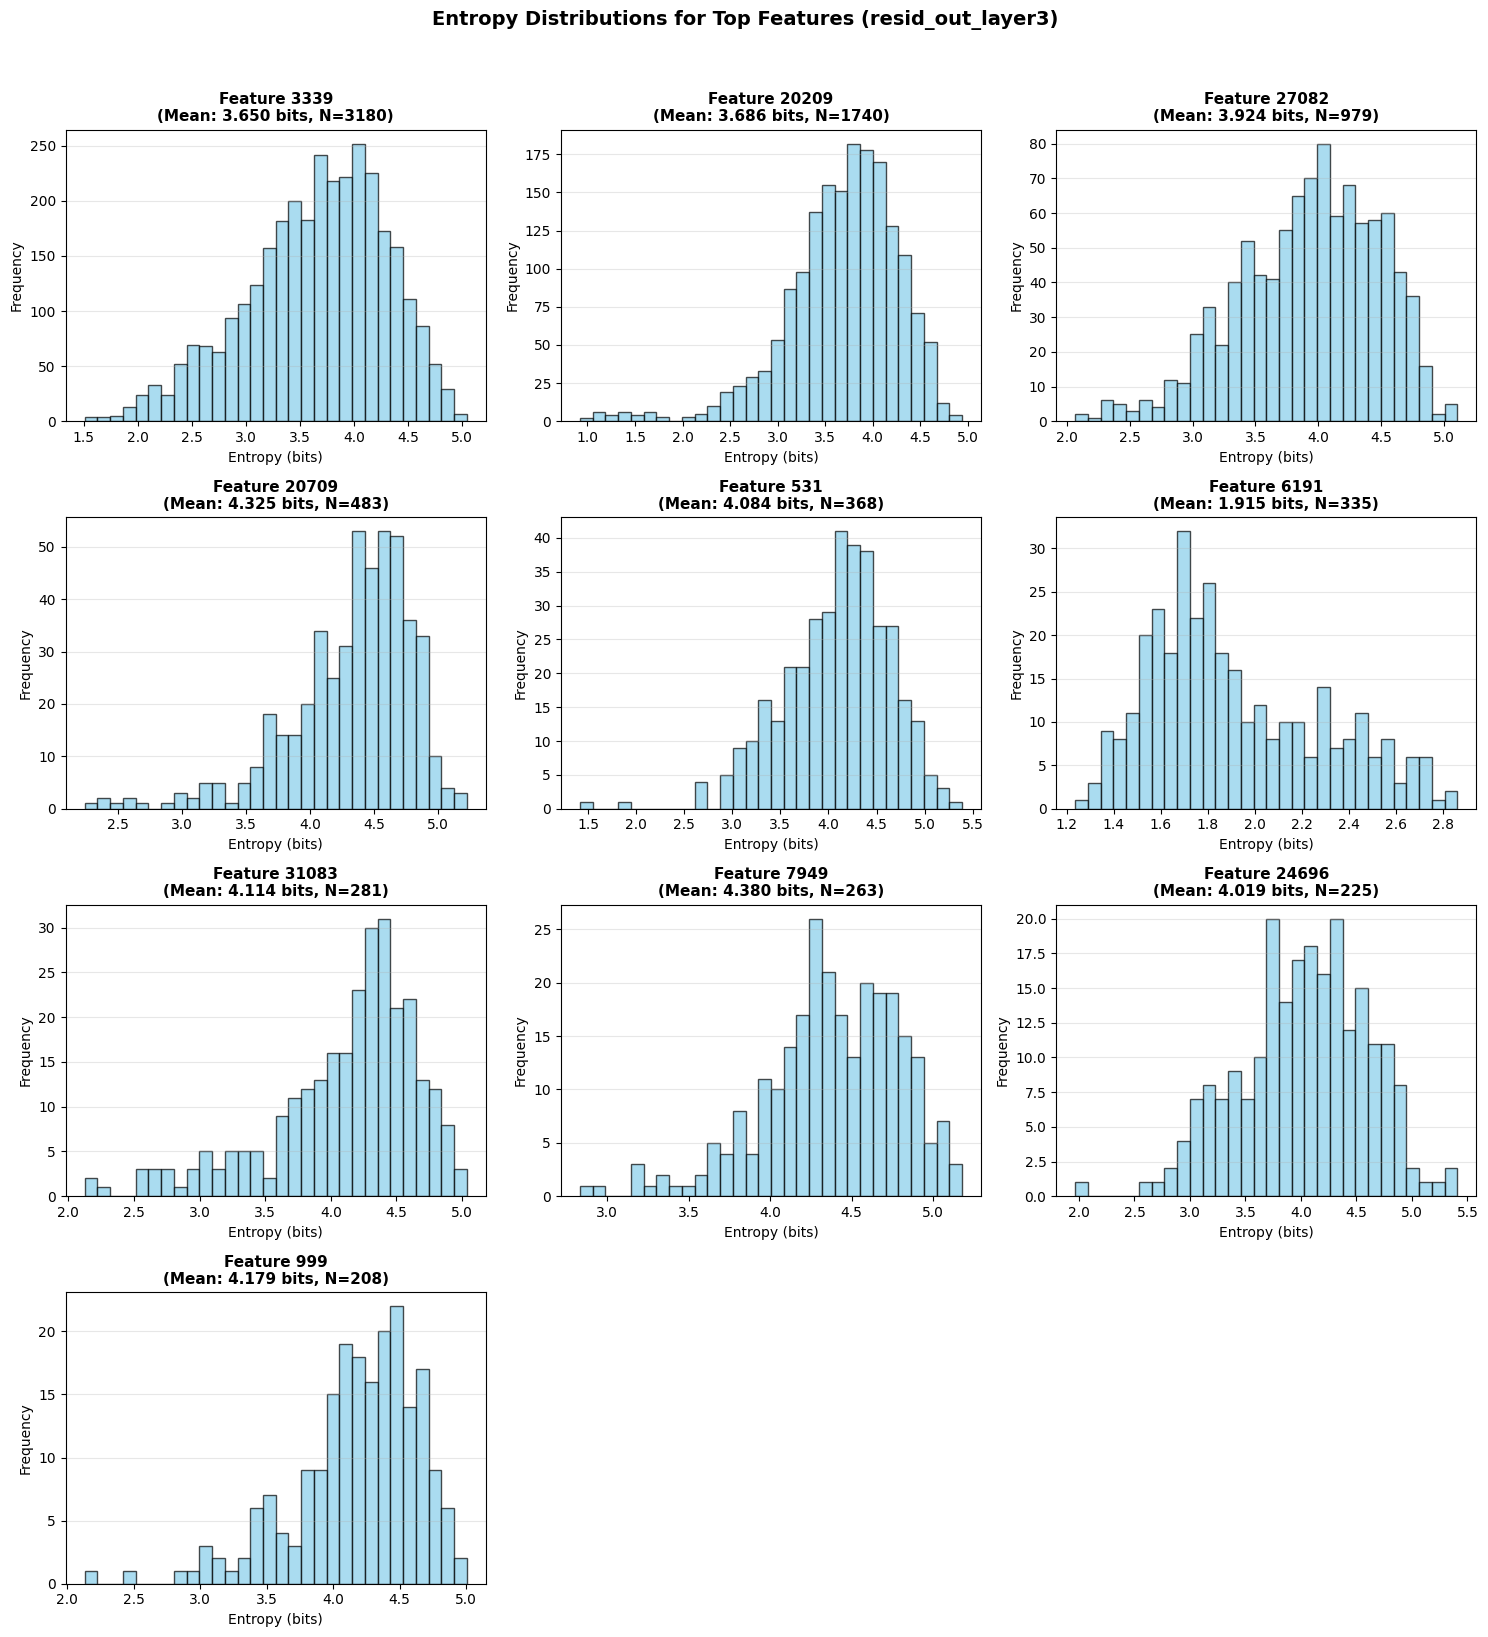
\includegraphics[width=\linewidth]{figures/entropy_distribution_batches.png}
    \caption{Entropy distributions across batches for top features at
        layer~3. Each panel shows the histogram of $S_a$ over all batches
        where the feature is active, with the mean entropy and number of
        samples~$N$ indicated. Mean entropies range from $1.915$~bits
        (Feature~6191, highly local) to $4.325$~bits (Feature~20709, highly
        nonlocal).}
    \label{fig:entropy_batches}
\end{figure}

\subsection{Depth dependence of entropy}
\label{sec:depth}

A key prediction of the holographic analogy is that features at deeper
layers should be more nonlocal, since deeper layers have access to more
tokens through the causal attention mechanism and encode more abstract
concepts.

Figure~\ref{fig:entropy_depth} shows the influence entropy as a function
of layer depth. Each gray dot represents one feature; colored lines track
selected features across layers. The red dashed line shows the token vector
entropy, and the blue dashed line shows the average entropy of the top-20
features at each layer. The average feature entropy increases monotonically
with depth.

\begin{figure}[t]
    \centering
    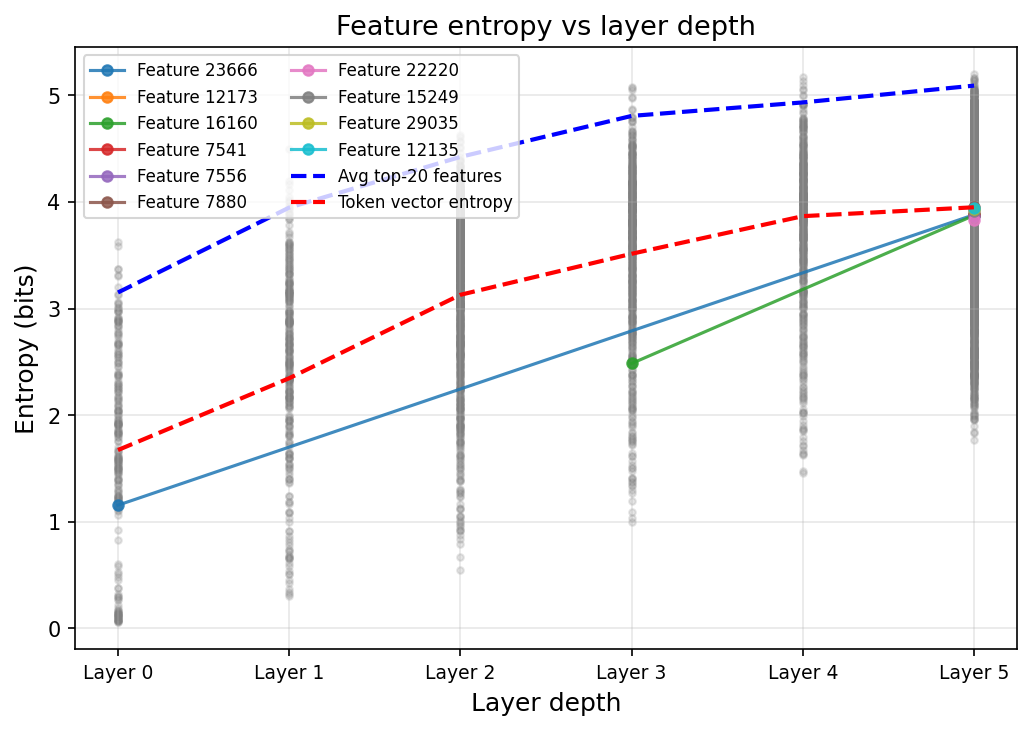
\includegraphics[width=0.58\linewidth]{figures/entropy_vs_depth.png}
    \caption{Feature entropy versus layer depth. Each gray dot is one
        feature; colored lines track selected features across layers. The red
        dashed line shows token vector entropy; the blue dashed line shows the
        average entropy of the top-20 features. Average entropy increases
        monotonically with layer depth, consistent with deeper layers encoding
        more nonlocal concepts.}
    \label{fig:entropy_depth}
\end{figure}

Figure~\ref{fig:entropy_histograms} provides another view: histograms of
the average feature entropy at each layer. The distribution shifts
progressively to higher entropy at deeper layers. Quantitatively, the mean
entropies (mean $\pm$ standard deviation) are:
layer~0: $0.898 \pm 0.618$~bits (71~features);
layer~1: $1.859 \pm 0.880$~bits (43~features);
layer~2: $2.484 \pm 0.922$~bits (116~features);
layer~3: $3.163 \pm 0.842$~bits (225~features);
layer~4: $3.705 \pm 0.809$~bits (211~features).
The number of leading features also increases with depth, reflecting the
increasing complexity of representations. The trend continues at layer~5,
where the mean entropy for 500~leading features is $4.054$~bits
(see Section~\ref{sec:comparison}).

\begin{figure}[t]
    \centering
    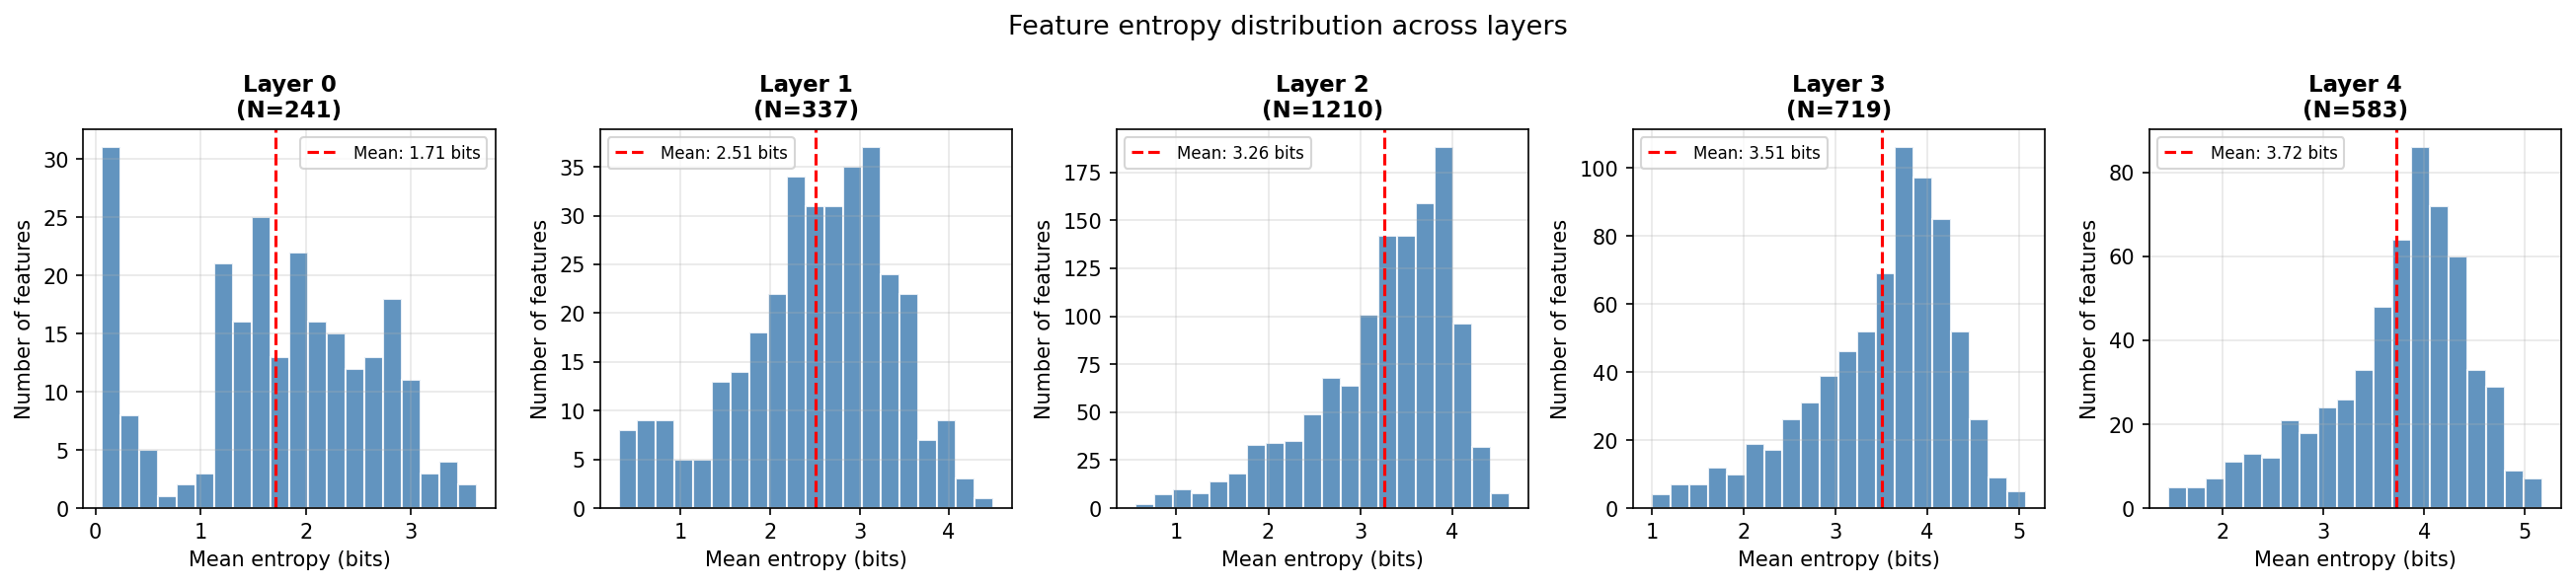
\includegraphics[width=0.52\linewidth]{figures/entropy_vs_activation_multilayer.png}
    \caption{Histograms of average feature entropy for leading features
        across layers~0--4. The number of leading features at each layer is
        indicated in parentheses. The distribution shifts to higher entropy at
        deeper layers, consistent with more abstract and nonlocal
        representations.}
    \label{fig:entropy_histograms}
\end{figure}

\subsection{Context length dependence}
\label{sec:length}

Figure~\ref{fig:entropy_length} shows the influence entropy as a function
of context length (batch size) for features at layer~2. As the context
length increases, feature entropies initially grow but saturate beyond
approximately 40--60~tokens. The saturation values are well below the
maximum possible entropy $\log_2 n$ (shown as a dashed line), confirming
that each feature has a finite effective support in token space. The
saturation value is feature-dependent and reflects the characteristic
nonlocality scale of each feature: some features saturate at
${\sim}1$~bit regardless of context length, while others reach
${\sim}4$~bits.

\begin{figure}[t]
    \centering
    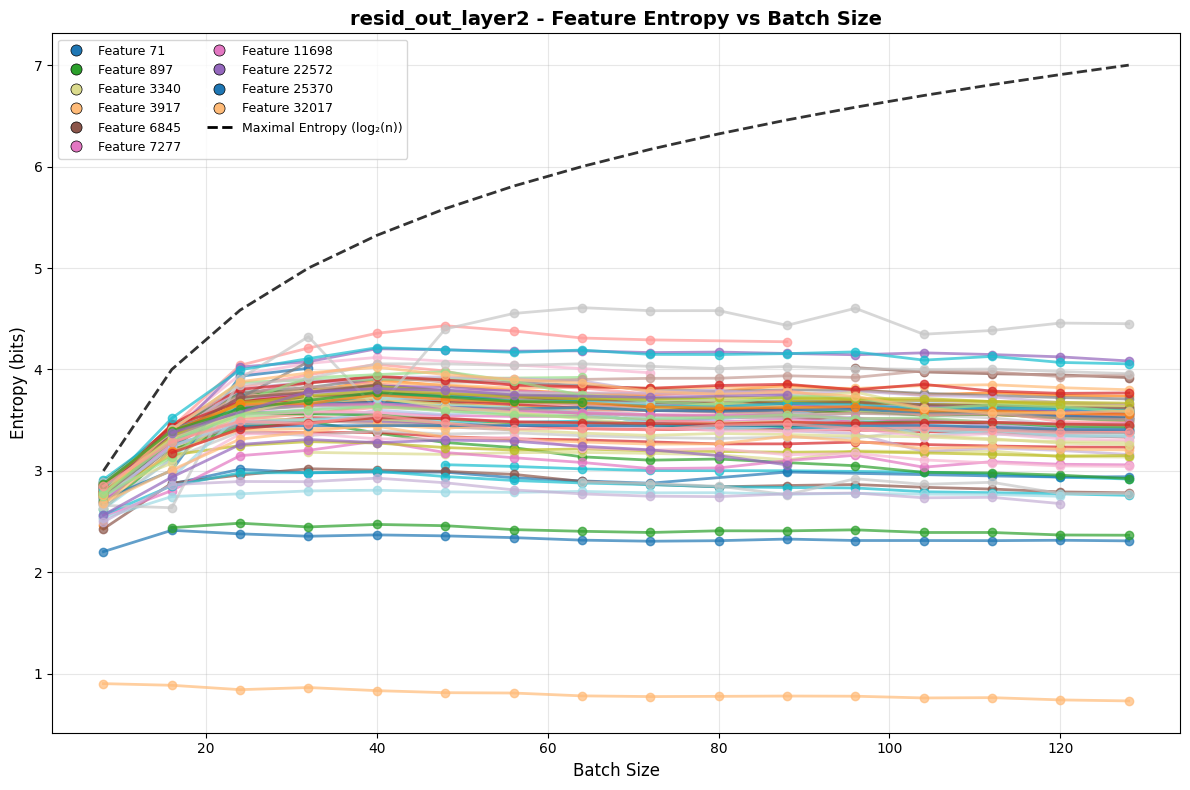
\includegraphics[width=0.78\linewidth]{figures/entropy_vs_batchsize.png}
    \caption{Feature entropy versus context length (batch size) for layer~2.
        Each curve corresponds to one leading feature. The dashed line shows
        the maximum possible entropy $\log_2 n$. Feature entropies saturate
        well below the maximum, indicating finite effective support.
        Highlighted features in the legend illustrate the range of saturation
        values.}
    \label{fig:entropy_length}
\end{figure}

\subsection{Feature versus token vector entropy}
\label{sec:comparison}

Finally, we compare the influence entropy of individual SAE features with
that of the reconstructed token vector $\tilde{y}$.
Figure~\ref{fig:entropy_activation} shows the averaged entropy versus
activation probability for 500~leading features at layer~5, with a mean
feature entropy of $4.054$~bits. In per-batch comparisons (e.g.,
Fig.~\ref{fig:entropy_depth}), the token vector entropy is indicated by a
dashed red line. At layer~4, the token vector entropy is approximately
$4.435$~bits, with most individual features falling below this value. At
layer~1, the token vector entropy is approximately $2.566$~bits, and again
most features have lower entropy.

\begin{figure}[t]
    \centering
    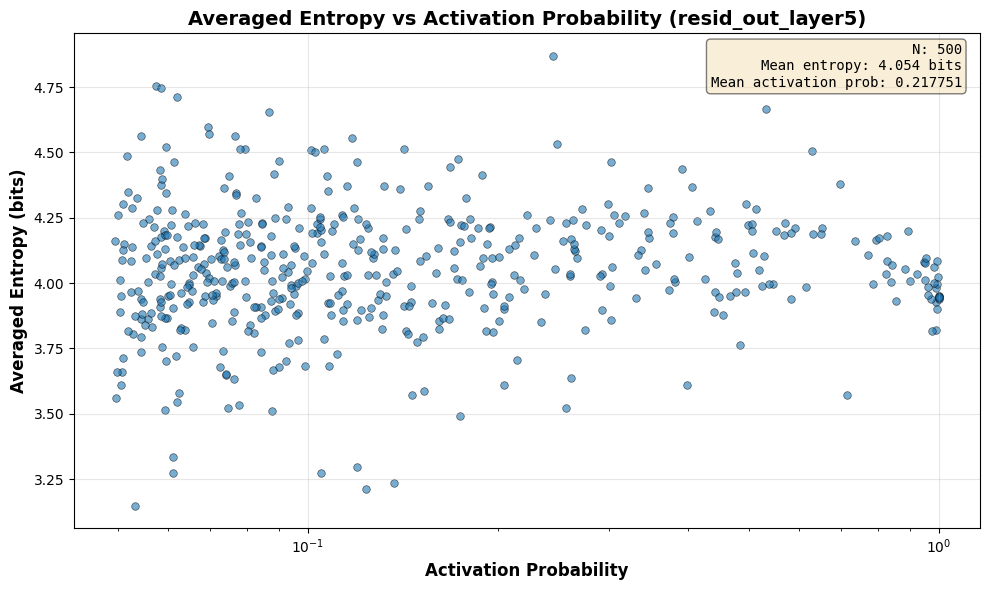
\includegraphics[width=0.72\linewidth]{figures/entropy_vs_activation.png}
    \caption{Averaged entropy versus activation probability for
        500~leading features at layer~5. The mean entropy is $4.054$~bits.
        Entropy is broadly distributed and does not depend strongly on
        activation frequency.}
    \label{fig:entropy_activation}
\end{figure}

These results are broadly consistent with the interpretation that the token
vector is a superposition of features with different nonlocality scales,
and that decomposing into SAE features yields a ``low-entropy
decomposition.'' However, the effect is not perfectly consistent across all
features: some individual features can have entropy comparable to or
exceeding that of the token vector, particularly at deeper layers where
both feature and token vector entropies are high. A more systematic
understanding of which features violate this pattern remains an open
question.

%=============================================================================
\section{Discussion and conclusion}
\label{sec:conclusion}
%=============================================================================

We have introduced a gradient-based entropy measure that quantifies the
nonlocality of sparse autoencoder features in the input token space of a
transformer language model. Our main findings are:

\begin{enumerate}
    \item \textbf{Nonlocality hierarchy.} SAE features exhibit a broad
          distribution of influence entropies, ranging from highly local
          (${\sim}1$~bit, effectively depending on one or two tokens) to highly
          nonlocal (${\sim}5$~bits, effectively depending on ${\sim}30$~tokens).
          This supports the picture that SAE features capture concepts at
          varying levels of abstraction.

    \item \textbf{Depth dependence.} Average feature entropy increases
          monotonically with layer depth, from $0.898$~bits at layer~0 to
          $3.705$~bits at layer~4. This is consistent with deeper layers
          encoding more abstract and context-dependent concepts, and is
          reminiscent of the radial dimension in holographic duality, where more
          nonlocal boundary operators correspond to bulk fields deeper in the
          geometry.

    \item \textbf{Context length saturation.} Feature entropy saturates with
          increasing context length, indicating that each feature has a
          characteristic nonlocality scale that is intrinsic to the feature
          rather than determined by the available context window.

    \item \textbf{Low-entropy decomposition.} Individual features generally
          have lower influence entropy than the full reconstructed token vector,
          supporting the view that SAE features decompose the residual stream
          into components with more structured dependence on the input.
\end{enumerate}

Several open questions merit further investigation. First, alternative
measures of nonlocality such as the participation ratio or R\'{e}nyi
entropies could provide complementary information about the structure of
the influence distribution. Second, it would be valuable to establish
criteria for when a feature extraction is ``good'' in terms of the entropy
distribution it produces---for example, whether minimizing the average
feature entropy subject to reconstruction accuracy leads to more
interpretable features. Third, it remains to be seen whether the patterns
we observe are universal across model scales and architectures. Fourth,
cross-layer SAEs that share features across multiple
layers~\citep{shi2025layersharing, bussmann2025matryoshka} could reveal
dynamical nonlocality in both the token and layer dimensions, potentially
giving a richer picture of the emergent geometry. Fifth, the logical
relations between features at different abstraction levels remain poorly
understood, and recent work has highlighted potential pitfalls such as
feature splitting, absorption, and hedging in narrow
SAEs~\citep{chanin2024absorption, chanin2025hedging}.

More broadly, we believe that analyzing LLMs from the angle of information
theory and emergent geometry is a fruitful direction. The holographic
analogy, while imperfect, provides a useful conceptual framework for
thinking about the structure of learned representations. The entropy
measure introduced here is a first step toward making this analogy
quantitative, and we hope it will inspire further connections between
theoretical physics and the interpretability of neural networks.

%=============================================================================
\begin{ack}
    We thank Aditya Cowsik, Kfir Dolev, and Bruno de Luca for valuable
    discussions. This work was supported in part by the Simons Foundation.
\end{ack}

\bibliographystyle{plainnat}
\bibliography{references}

%=============================================================================
\appendix
\section{Details of the gradient computation}
\label{app:gradients}

The influence matrix in Eq.~\eqref{eq:influence_matrix} is computed using
PyTorch automatic differentiation. For each batch of $L$~tokens, we
perform a forward pass through the transformer with gradient tracking
enabled on the input embeddings. The embedding layer is temporarily
replaced with a fixed tensor to ensure that the input embeddings are leaf
variables in the computation graph, so that
$\partial f_a / \partial x_{\mu,t'}$ is well defined.

For feature influences, we compute
$\partial f_a(L,n) / \partial x_{\mu,t'}$ via
\texttt{torch.autograd.grad} with \texttt{retain\_graph=True} for each
active feature~$a$ at the last token position. The squared norm
(Eq.~\eqref{eq:influence_strength}) is computed from the resulting
gradient tensor of shape $[1, L, d_{\mathrm{model}}]$. For token vector
influences, we use \texttt{torch.autograd.functional.jacobian} to compute
the full Jacobian
$\partial \tilde{y}_\nu(L,n) / \partial x_{\mu,t'}$ of shape
$[d_{\mathrm{model}}, L, d_{\mathrm{model}}]$ in a single vectorized
call. The token influence $R(t,n \mid t')$ is then obtained by summing
the squared Jacobian over the output and input component indices.

All experiments were conducted on Apple M-series hardware using the MPS
backend, with typical processing times of ${\sim}0.5$~seconds per batch
for feature influences and ${\sim}2$~seconds per batch for the full
Jacobian computation.

\end{document}
